\documentclass{article}
\usepackage[utf8]{inputenc}
\title{Dynamic Model in the Proximal tubule of Rat Kidney}
\author{Jing Yang}
\date{November 2019}

\usepackage{natbib}
\usepackage{graphicx}
\usepackage{amsmath}
\usepackage{float}


\begin{document}

\maketitle

\begin{abstract}
We developed a dynamic model of a male rat proximal tubule in order to investigate results brought by changes on different lumen boundary conditions. We examined how long it will take to reach a steady state again from a sudden change. We also investigated whether oscillation on a single parameter will result in similar oscillations on other parameters. We determined that these oscillations will not have a significant passive effect on proximal tubule's re-absorption. We also noticed several irregular phenomenon such as phase difference and amplitude difference on the oscillation pattern of concentrations in different part along the tubule. And we tried to explain these response by using physiological knowledge.\\

\noindent \textbf{Keywords: }Proximal tubule $\cdot$ Oscillations $\cdot$ Concentrations $\cdot$ Dynamic model
\end{abstract}


\section{Model Formulation}
In proximal tubule, cells and tight junctions between cells form a single-layer cell wall between lumen and bath. We build our model based on the steady state model that Anita Layton published\citep{layton2014mathematical}. The model consider fifteen kinds of solutes, including $\rm {Na}^{+}$,$\rm {K}^{+}$,$\rm {Cl}^{-}$,$\rm {HCO}_{3}^{-}$,$\rm H_{2}CO_{3}$,$\rm CO_{2}$,$\rm HPO_{4}^{2-}$,$\rm H_{2}PO_{4}^{-}$,urea,$\rm NH_{3}$,$\rm NH_{4}^{+}$,$\rm H^{+}$,\\$\rm HCO_{2}^{-}$,$\rm H_{2}CO_2$ and glucose. Model contains four compartments (Lumen, cell, lateral space, bath).Solutes are exchanged between different compartments through diffusion, transporters and coupled transporters. System equations are based on mass conservation and electronic neutrality. 


\subsection{Water Conservation}
Water conservation in cell and lateral space (denoted by subscripts ``C'' and ``P'' respectively) is given by\citep{edwards2017cell}:\\
\begin{equation}
\frac{\mathrm{d} V_{\mathrm{C}}}{\mathrm{d} t}=J_{v, \mathrm{LC}}+J_{v, \mathrm{BC}}+J_{v, \mathrm{PC}}
\end{equation}
\begin{equation}
\frac{\mathrm{d} V_{\mathrm{p}}}{\mathrm{d} t}=J_{v, \mathrm{LP}}+J_{v, \mathrm{BP}}+J_{v, \mathrm{CP}}
\end{equation}
where the subscripts ``L'' and ``B'' denote lumen and bath respectively, and ``v'' denotes volume of water. Water conservation in lumen is given by:
\begin{equation}
0=-\frac{\partial \mathrm{F}_{v}}{\partial x}+2 \pi r (J_{v,\mathrm{CL}}+J_{v,\mathrm{PL}})
\end{equation}
where $\mathrm{F}_{v}$ means water flow in lumen, $r$ means radius of lumen and partial derivative means along the lumen.

\subsection{Solute Conservation}
For non-reacting solute $k$, conservation equations are given by:
\begin{equation}
\frac{\mathrm{d} V_{\mathrm{C}} C_{k, \mathrm{C}}}{\mathrm{d} t}=J_{k, \mathrm{LC}}+J_{k, \mathrm{BC}}+J_{k, \mathrm{PC}}
\end{equation}
\begin{equation}
\frac{\mathrm{d} V_{\mathrm{P}} C_{k, \mathrm{P}}}{\mathrm{d} t}=J_{k, \mathrm{LP}}+J_{k, \mathrm{BP}}+J_{k, \mathrm{CP}}
\end{equation}
\begin{equation}
0=-\frac{\partial\left(\mathrm{F}_{v} C_{k,\mathrm{L}}\right)}{\partial x}+2 \pi r (J_{k,\mathrm{CL}}+J_{k,\mathrm{PL}})
\end{equation}
where $C_{k,i}$ denotes the concentration of solute $k$ in compartment $i$ and $J_{k,ij}$ denotes flux of solute $k$ from compartment $i$ to $j$.\\

For the reacting solutes, conservation is applied to the total buffers. Take the buffer $\mathrm{HPO}_{4}^{2-} and {H}_{2} \mathrm{PO}_{4}^{-}$ for instance:
\begin{equation}
\frac{\mathrm{d}}{\mathrm{d} t}\left(V_{i}\left(C_{\mathrm{HPO}_{4}^{2-}, i}+C_{\mathrm{H}_{2} \mathrm{PO}_{4}^{-}, i}\right)\right)=\hat{J}_{\mathrm{HPO}_{4}^{2-}, i}+\hat{J}_{\mathrm{H}_{2} \mathrm{PO}_{4}^{-}, i}
\end{equation}
where $i$ corresponding to C or P. $\hat{J}_{k, i}$ denotes the net flux of solute k into the compartment i.
\begin{equation}
\frac{\mathrm{d}}{\mathrm{d} t}\left(F_{v}\left(C_{\mathrm{HPO}_{4}^{2-}, L}+C_{\mathrm{H}_{2} \mathrm{PO}_{4}^{-}, L}\right)\right)=\hat{J}_{\mathrm{HPO}_{4}^{2-}, L}+\hat{J}_{\mathrm{H}_{2} \mathrm{PO}_{4}^{-}, L}
\end{equation}
The other buffer pairs $\left(\mathrm{CO}_{2},\mathrm{HCO}_{3}^{-}, \mathrm{H}_{2} \mathrm{CO}_{3}\right),\left(\mathrm{HPO}_{4}^{2-}, \mathrm{H}_{2} \mathrm{PO}_{4}^{-}\right),\left(\mathrm{NH}_{3}, \mathrm{NH}_{4}^{+}\right)$ all have above equations.
The buffer pairs are in equilibrium:
\begin{equation}
\mathrm{pH}=\mathrm{pK}_{A}-\log \frac{C_{A, i}}{C_{B, i}}
\end{equation}
where the buffer pairs (A,B) are $\left(\mathrm{HCO}_{3}^{-}, \mathrm{H}_{2} \mathrm{CO}_{3}\right),\left(\mathrm{HPO}_{4}^{2-}, \mathrm{H}_{2} \mathrm{PO}_{4}^{-}\right),\left(\mathrm{NH}_{3}, \mathrm{NH}_{4}^{+}\right),\left(\mathrm{HCO}_{2}^{-}, \mathrm{H}_{2} \mathrm{CO}_{2}\right)$.
The conservation of hydrogen is given by:
\begin{equation}
\begin{aligned}
\frac{\mathrm{d}}{\mathrm{d} t}\left(V_{i} (C_{\mathrm{H}^{+}}+C_{\mathrm{NH}_{4}^{+}}-C_{\mathrm{HCO_{3}^{-}}}-C_{\mathrm{HPO_{4}^{2-}}}-C_{\mathrm{HCO_{2}^{-}}}) \right)\\=\sum (\hat{J}_{H^{+}, i}+\hat{J}_{\mathrm{NH}_{4}^{+}, i}-\hat{J}_{ \mathrm{HCO_{3}^{-}, i}}-\hat{J}_{ \mathrm{HPO_{4}^{2-}, i}}-\hat{J}_{ \mathrm{HCO_{2}^{-}, i}})
\end{aligned}
\end{equation}

\section{Calculation}
We discrete time-dependent term by Back-Euler Method. For the partial differential term, we simply regard $F_{v}$ does not change too much along one cell's length along the tubule. For instance, solute conservation equation in lumen can be discrete as following:
For non-reacting solute $k$, conservation equations are given by:
\begin{equation}
\frac{V_{\mathrm{C}}^{n+1} C_{k, \mathrm{C}}^{n+1}-V_{\mathrm{C}}^{n} C_{k, \mathrm{C}}^{n}}{\Delta t}=J_{k, \mathrm{LC}}^{n+1}+J_{k, \mathrm{BC}}^{n+1}+J_{k, \mathrm{PC}}^{n+1}
\end{equation}
where ${\Delta t}$ means time step length, superscript $n$ means the n-th time step.

\section{Discovery}
After finishing the building of dynamic model, we can do various numerical experiments to observe changes along the time. In general, we did four kinds of experiments on boundary conditions separately :
\begin{itemize}
	\item Increase a certain solute concentration level
	\item Add various frequency and amplitude oscillations on single nephron glomerular filtration rate (SNGFR) 
	\item Add various frequency and amplitude oscillations a certain solute concentration
	\item Add oscillations on solute concentration and SNGFR simultaneously
\end{itemize}
And we found several interesting results and tried to explain them by physiological knowledge.

\subsection{Recover Time}
We increase glucose and urea concentration in lumen boundary condition separately. The proximal tubule plays an important role in re-absorption. Glucose are transported through transporter SGLT2 between lumen and cell,through transporter GLUT2 between cell and bath. Urea is a kind of inorganic chemicals with small molecule. It is transported by diffusion. Glucose and urea are both chemicals with no valence, meanwhile their concentrations are close in lumen. We calculate the convergence process to exam their difference in re-absorption. The transporter will accelerate the re-absorption process, thus we expect that the former experiment will reach the balance more quickly. Since we assume that lumen is incompressible, thus lumen concentrations will react to the sudden change almost simultaneously. Thus we observe cellular concentrations to judge the convergence. We find in both experiments the tubule will recover to steady state in 10-15 seconds. Moreover, if we increase other kind of solutes in similar scales, they can all reach the balance in 20 seconds. It indicates that the proximal tubule have the ability of reacting to the changes in boundary conditions quickly and keeping the lumen environment in steady state.

\begin{figure}[H]
\centering
\begin{minipage}[t]{0.48\textwidth}
\centering
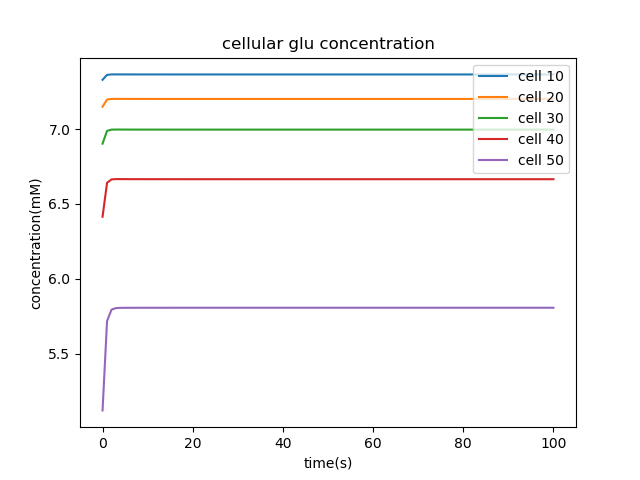
\includegraphics[width=6cm]{figure/figure1.png}
\caption{Glucose concentration}
\end{minipage}
\begin{minipage}[t]{0.48\textwidth}
\centering
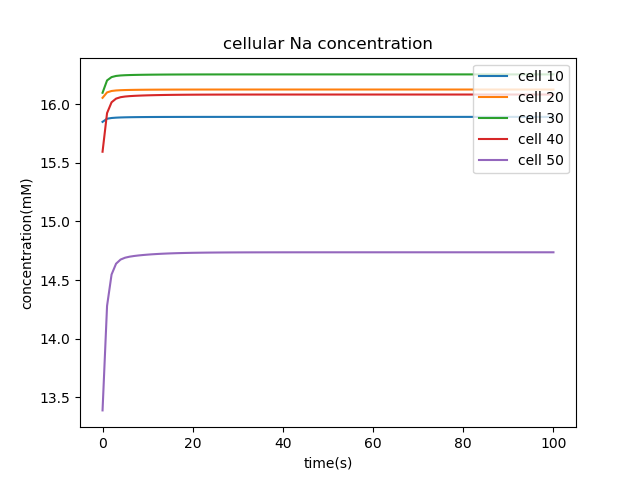
\includegraphics[width=6cm]{figure/figure2.png}
\caption{Sodium concentration}
\end{minipage}
\end{figure}

Figure 1 and Figure 2 is cellular glucose and sodium concentration trend after we increasing lumen boundary glucose concentration by 10\%.

\begin{figure}[H]
\centering
\begin{minipage}[t]{0.48\textwidth}
\centering
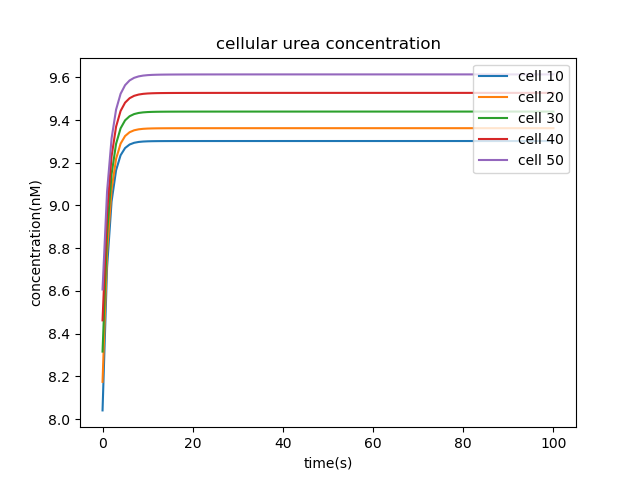
\includegraphics[width=6cm]{figure/figure3.png}
\caption{urea concentration}
\end{minipage}
\begin{minipage}[t]{0.48\textwidth}
\centering
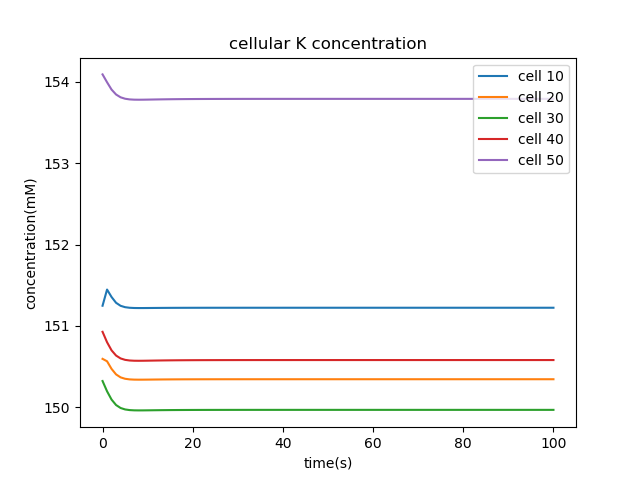
\includegraphics[width=6cm]{figure/figure4.png}
\caption{Potassium concentration}
\end{minipage}
\end{figure}
Figure 3 and Figure 4 is urea glucose and potassium concentration trend after we increasing lumen boundary urea concentration by 10\%.

\subsection{Oscillation on SNGFR}
Experiments show that SNGFR has an oscillation of about 30 seconds time period. We include this oscillations in our numerical experiments to exam whether the oscillations will affect the tubule re-absorption function. We add oscillations as following form:
\begin{equation}
\mathrm{SNGFR}(t)=\mathrm{SNGFR}^{0}*(1+Asin(\frac{2\pi t}{T} ))
\end{equation}
where $SNGFR^{0}$ means original SNGFR baseline, A and T denote amplitude and time period separately. We choose T as 15, 30 or 60, A as 0.1, 0.3 or 0.5 in the experiment.

\begin{figure}[H]
\centering
\begin{minipage}[t]{0.48\textwidth}
\centering
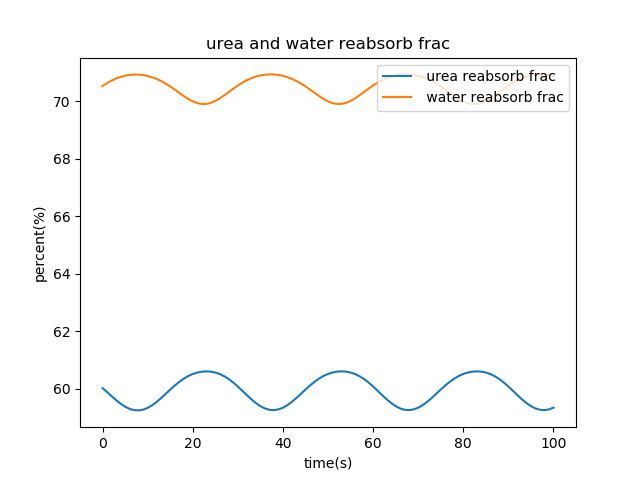
\includegraphics[width=6cm]{figure/figure5.png}
\caption{T=30 A=0.1}
\end{minipage}
\begin{minipage}[t]{0.48\textwidth}
\centering
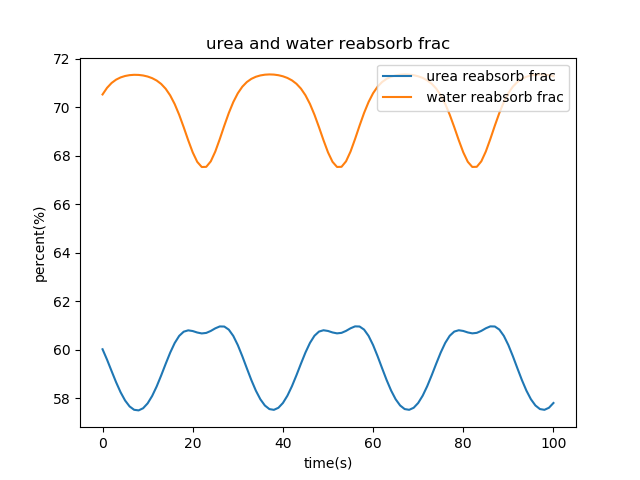
\includegraphics[width=6cm]{figure/figure6.png}
\caption{T=30 A=0.3}
\end{minipage}
\end{figure}

\begin{figure}[H]
\centering
\begin{minipage}[t]{0.48\textwidth}
\centering
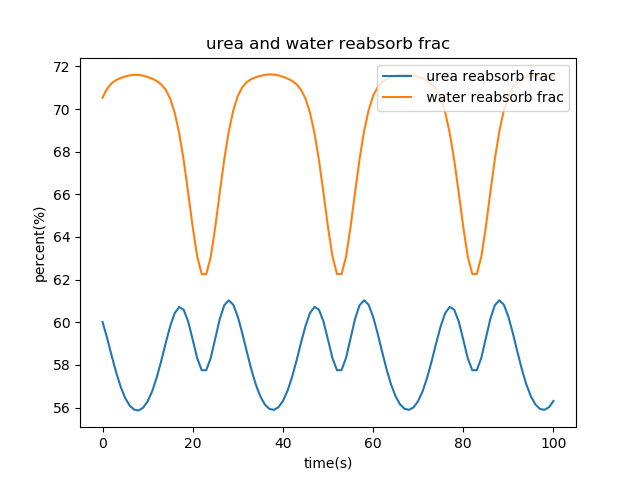
\includegraphics[width=6cm]{figure/figure7.png}
\caption{T=30 A=0.5}
\end{minipage}
\begin{minipage}[t]{0.48\textwidth}
\centering
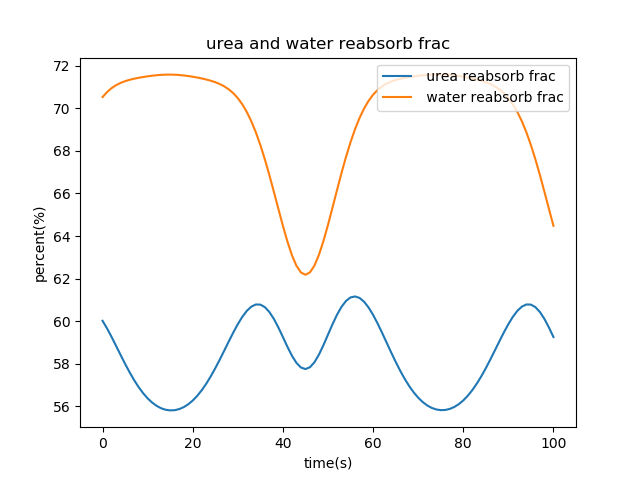
\includegraphics[width=6cm]{figure/figure8.png}
\caption{T=60 A=0.5}
\end{minipage}
\end{figure}

We observe urea re-absorption fraction instead of glucose since the fraction of glucose is over 99.7\%, oscillations are too small to be noticed. Figure 5-8 are urea and water re-absorption fraction with respect to time in different T and A. We find that though we add up to 50\% oscillation on SNGFR, the re-absorption of water and urea oscillate no more than 5\%, which suggests that proximal tubule re-absorption function keeps in a respectively stable state with the change of SNGFR. And we also notice the sudden drop in the fraction patterns of urea when oscillations over 30\% of the baseline. We observe similar pattern of dropping in T=30 and 60, suggesting it can not be attributed to not having enough time to transport solute when SNGFR is high. The dropping can be explained by that the re-absorption ability of urea reaches maximum when SNGFR over 1.3 times of baseline. 

\subsection{Damping}
Proximal tubule plays an important role in damping, which guarantees a stable environment for nephron to work. We add an oscillation to a particular kind of solute to verify it. We oscillate NaCl concentration in boundary condition as following form:
\begin{equation}
\mathrm{C_{NaCl}}(t)=\mathrm{C_{NaCl}}^{0}+A*sin(\frac{2\pi t}{T})
\end{equation} 
where we choose A as 20 mM, T as 30 seconds.
\begin{figure}[H]
\centering
\begin{minipage}[t]{0.48\textwidth}
\centering
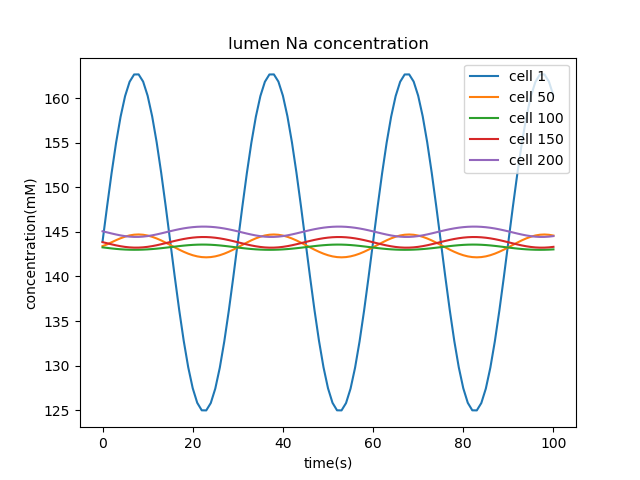
\includegraphics[width=6cm]{figure/figure9.png}
\caption{$Na^{+}$ concentration}
\end{minipage}
\begin{minipage}[t]{0.48\textwidth}
\centering
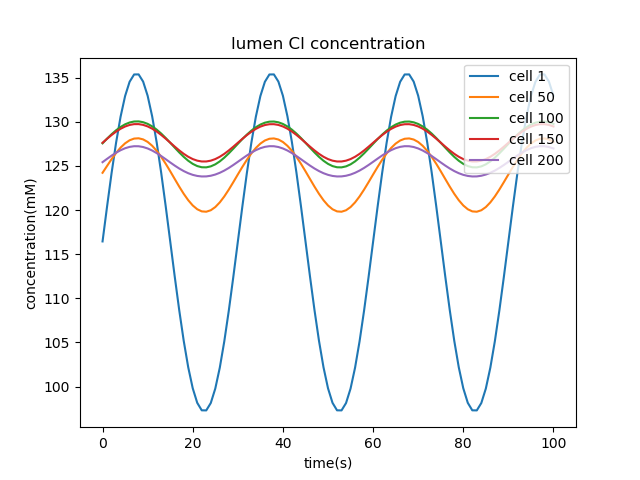
\includegraphics[width=6cm]{figure/figure10.png}
\caption{$Cl^{-}$ concentration}
\end{minipage}
\end{figure}

\begin{figure}[H]
\centering
\begin{minipage}[t]{0.48\textwidth}
\centering
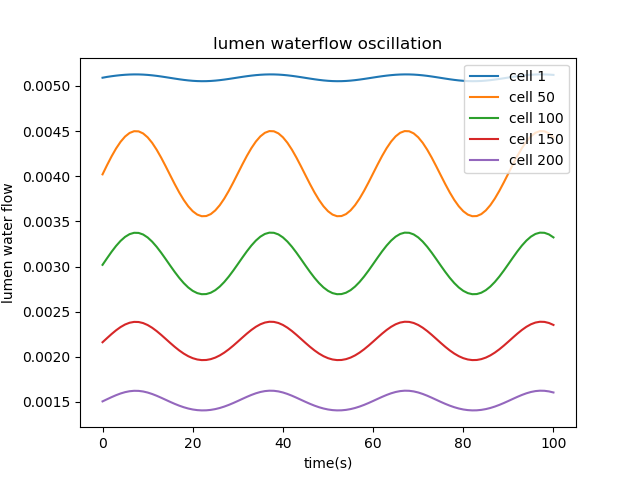
\includegraphics[width=6cm]{figure/figure11.png}
\caption{Water flow oscillation}
\end{minipage}
\begin{minipage}[t]{0.48\textwidth}
\centering
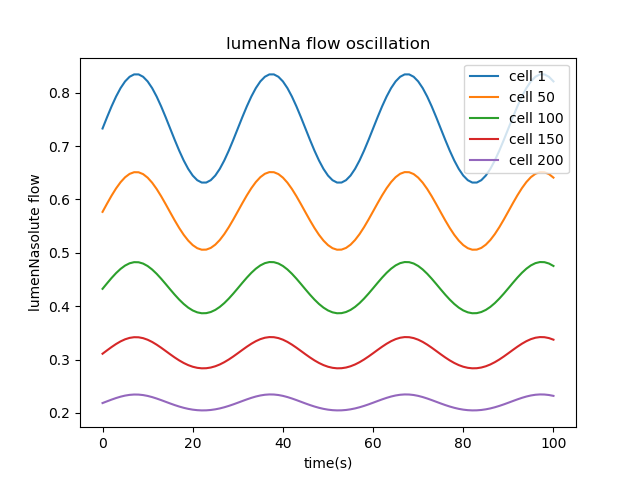
\includegraphics[width=6cm]{figure/figure12.png}
\caption{$Na^{+}$ flow oscillation}
\end{minipage}
\end{figure}
From Figure 9 and 10 we can see the obvious damping on the concentration of $Na^{+}$ and $Cl^{-}$. Figure 12 also verify it by plotting the solute flow in lumen. Figure 11 is water flow in lumen. At the beginning of the tubule, the amplitude of water flow oscillation will increase due to the oscillation of $NaCl$ concentration. The amplitude decreases later on. Such damping can be also found when we add oscillation on boundary water flow separately.

\subsection{Phase Difference}
When we add on oscillation on $NaCl$ concentration as following form:
\begin{equation}
\mathrm{C_{NaCl}}(t)=\mathrm{C_{NaCl}}^{0}+20*sin(\frac{2\pi t}{30})
\end{equation} 
we found a phase difference in lumen potassium concentration. Such difference can be also observed in other solutes more or less.
\begin{figure}[H]
\centering
\begin{minipage}[t]{0.48\textwidth}
\centering
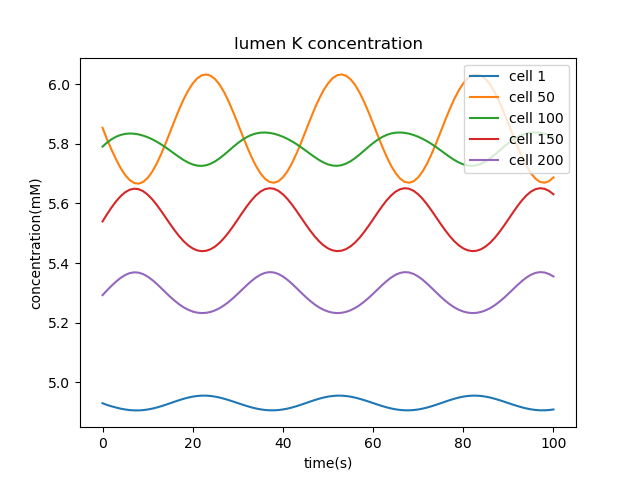
\includegraphics[width=6cm]{figure/figure13.png}
\caption{$K^{+}$ phase difference}
\end{minipage}
\begin{minipage}[t]{0.48\textwidth}
\centering
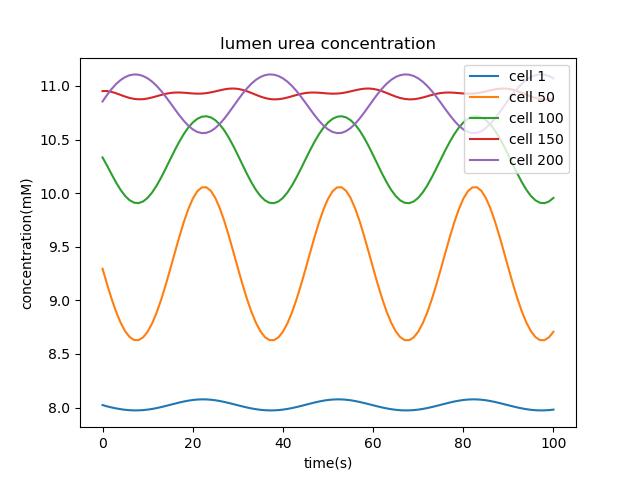
\includegraphics[width=6cm]{figure/figure14.png}
\caption{Urea phase difference}
\end{minipage}
\end{figure}
It can be explained by that the concentrations of all solutes are not monotonous along the tubule. And if we change the concentration of NaCl, different part of tubule will behave differently on the trend of concentration changes. Figure 15 and 16 show lumen and cellular potassium concentration trend along the tubule for the few seconds.
\begin{equation}
\mathrm{C_{NaCl}}(t)=\mathrm{C_{NaCl}}^{0}+20*sin(\frac{2\pi t}{30})
\end{equation} 
we found a phase difference in lumen potassium concentration. Such difference can be also observed in other solutes more or less.
\begin{figure}[H]
\centering
\begin{minipage}[t]{0.48\textwidth}
\centering
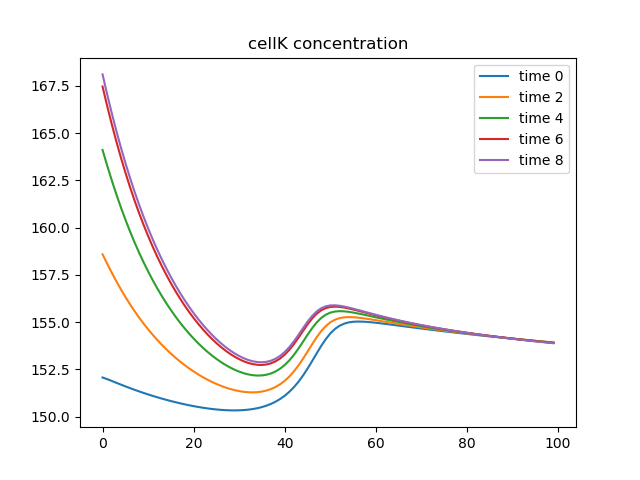
\includegraphics[width=6cm]{figure/figure15.png}
\caption{Lumen $K^{+}$}
\end{minipage}
\begin{minipage}[t]{0.48\textwidth}
\centering
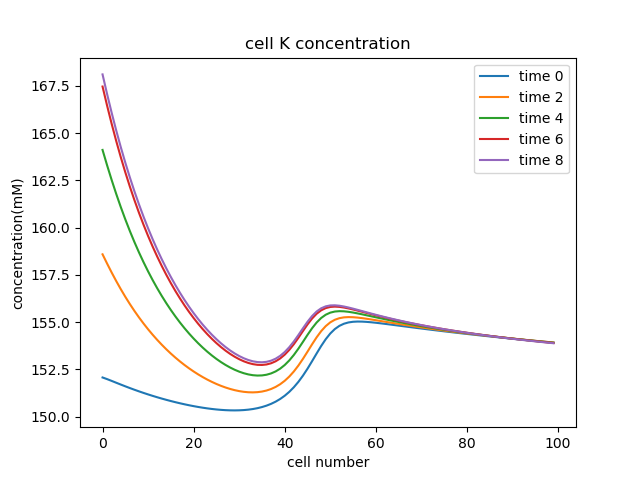
\includegraphics[width=6cm]{figure/figure16.png}
\caption{Cellular $K^{+}$}
\end{minipage}
\end{figure}

And the transportation of potassium is completed by diffusion, channels and transporters, which is most decided by potential difference and concentration difference. The different changing trend will account for different potassium net flux in lumen (Figure 17 and 18). From the plotting we can conclude some parts of the tubule transports solute (potassium or urea) from lumen to cell while others are opposite, which results in the phase difference.
\begin{figure}[H]
\centering
\begin{minipage}[t]{0.48\textwidth}
\centering
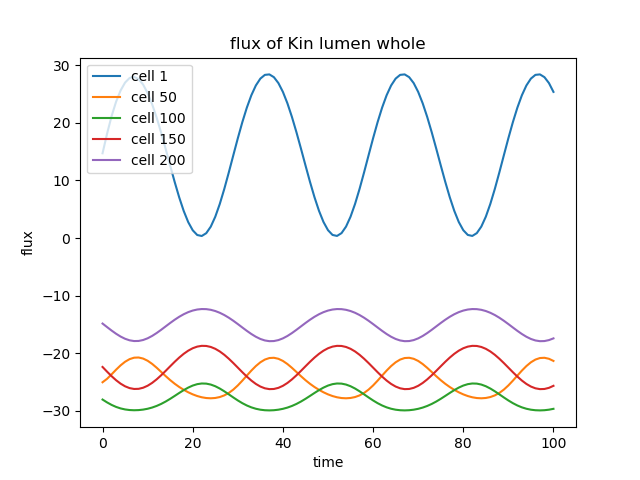
\includegraphics[width=6cm]{figure/figure17.png}
\caption{Lumen $K^{+}$ net flux}
\end{minipage}
\begin{minipage}[t]{0.48\textwidth}
\centering
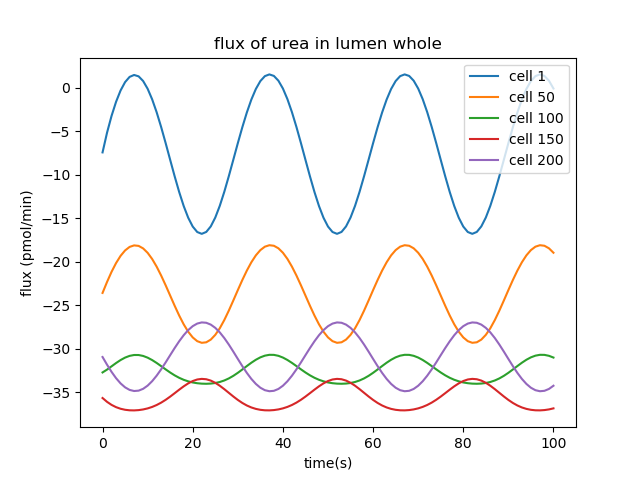
\includegraphics[width=6cm]{figure/figure18.png}
\caption{Lumen urea net flux}
\end{minipage}
\end{figure}
Such phase difference can be observed in all kind of solutes and cellular volume. Similar explanation can be applied.

\section{Discussion}
Since the dynamic data is quite hard to measure, we can not compare our numerical experiment with reality. A relatively stable environment is quite important for proximal tubule to play its functions. We show that proximal tubule react quickly to the changes and have the ability of damping the oscillations. That suggests the proximal tubule have a negative feedback mechanism to adjust solute concentrations, which plays an important role in concentration adjustment.


\bibliographystyle{plain}
\bibliography{references}
\end{document}
